\section{Lemmata}

\begin{frame}{\FrameName}
\begin{block}{Lemma 1}
  \begin{center}
    \fbox{
      $
      m^* \in \Omega(log(n))
      $
    }
  \end{center}
  \begin{center}
    \Hint{(Ohne Beweis)}
  \end{center}
  
\end{block}
\end{frame}

\begin{frame}{\FrameName}
\begin{block}{Lemma 2a}
  \begin{center}
    \fbox{
      Es gibt Grammatik der Größe $|G_\alpha| + |G_\beta| + 2$ für $\alpha \beta$.
    }
  \end{center}
  \begin{itemize}
    \item<2-> $G_\alpha$ und $G_\beta$ vereinigen
    \item<3-> Neue Startregel: $S \rightarrow S_\alpha S_\beta$
  \end{itemize}
  
\end{block}
\end{frame}

\begin{frame}{\FrameName}
  \begin{block}{Lemma 2b}
    \begin{center}
      \fbox{
        Es gibt Grammatik der Größe $|G_\alpha| + \mathcal{O}(log(k))$ für $\alpha^k$.
      }
    \end{center}
    \begin{itemize}
      \item<2-> Neue Regeln baumartig strukturieren
      \item<3-> Baum hat nur logarithmische Höhe
    \end{itemize}
    \visible<4->{
      
      \begin{minipage}[h]{0.3\textwidth} 
        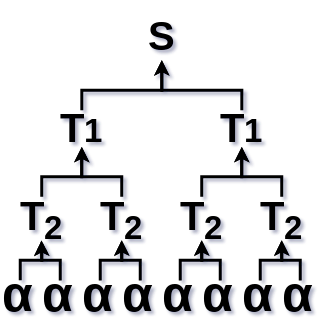
\includegraphics[width=\textwidth]{Images/Definitions/Tree.png}
     \end{minipage}
     \begin{minipage}[h]{0.5\textwidth}
      $$S \rightarrow T_1 T_1 $$
      $$T_1 \rightarrow T_2 T_2 $$
      $$T_2 \rightarrow \alpha \alpha $$
     \end{minipage}
    }

    
  \end{block}
    \end{frame}

\begin{frame}{\FrameName}
  \begin{block}{Lemma 3 \Hint{(mk-Lemma)}}
    \begin{center}
      \fbox{\begin{tabular}{@{}c@{}}
        In einem String gibt es maximal $mk$ \underline{unterschiedliche} \\ Substrings der Länge $k$
      \end{tabular}}
    \end{center}

    \begin{center}
      \Hint{(Ohne Beweis)}
    \end{center}
    
  \end{block}
  \end{frame}

